\laborator{Регрессионный анализ, методы аппроксимации}

\goal ознакомится с возможностями математического пакета Mathcad при решении задач регрессионного анализа; ознакомится с процедурами численного решения алгебраических уравнений и систем уравнений, реализованными в данном пакете. 

\subsection*{Теория}
Регрессионный анализ --- статистический метод исследования зависимости между зависимой переменной $y$ и одной или несколькими независимыми переменными $x_1$,$x_2$,...,$x_n$.
В статистике для оценки силы корреляционной зависимости двух случайных величин используется коэффициент корреляции $r_{xy}$. Определяется он отношением математического ожидания произведения отклонений случайных величин от их средних значений к произведению среднеквадратичных отклонений этих величин:
\begin{equation}
	r_{xy}=\dfrac{\dfrac{1}{n} \sum\limits_{i=1}^{n} (x_i-\bar{x}) (y_i-\bar{y}), }{\sigma_x \sigma_y}
\end{equation}
где $x$ и $y$ --- среднеквадратичные отклонения, определяемые следующим образом:
\begin{equation}
	\sigma_x=\sqrt{\dfrac{1}{n} \sum\limits_{i=1}^{n}(x_i-\bar{x})^2},
\end{equation}
где $\bar{x}=\dfrac{1}{n} \sum\limits_{i=1}^{n} x_i$.
Аналогичные выражения записываются и для $y$.

В Mathcad коэффициент корреляции двух выборок по данной формуле можно подсчитать с помощью встроенной функции \mc{corr(x,y)} (где \mc{x} и \mc{y} --- векторы, между которыми определяется коэффициент корреляции). Если коэффициент корреляции равен по модулю единице, то между случайными величинами существует линейная зависимость. Если же он равен нулю, то случайные величины независимы. В случае промежуточных значений $r_{ху}$, зависимость $y$ от $x$ может быть нелинейной или иметь высокое значение шума.

Если две выборки коррелируют, то можно установить зависимость между ними. Для вычисления регрессии в Mathcad имеется ряд функций. Обычно эти функции создают кривую или поверхность определенного типа, которая минимизирует ошибку между собой и имеющимися данными. Функции отличаются прежде всего типом кривой или поверхности, которую они используют, чтобы аппроксимировать данные.

Конечный результат регрессии --- функция с набором параметров, с помощью которой можно оценить значения в промежутках между заданными точками. Расхождение полученной функции регрессии с экспериментальными данными можно оценить через относительную среднюю и максимальную ошибку:

\begin{equation}
	err_i= \dfrac{\left| y_i^э - y(x^э_i) \right|}{y_i^э} 100\ \% ,
\end{equation}
\begin{equation}
	err_{av}=\dfrac{1}{n}\sum\limits_{i=1}^{n} err_i ,
\end{equation}
где $y_i^э$, $y(x_i^э)$ --- экспериментальное и расчетное значение функции; $n$ --- число экспериментальных точек; $err_i$ --- ошибка в i–й точке (из них определяется максимальная); $err_{av}$ --- средняя ошибка функции регрессии.

В Mathcad имеются встроенные функции для определения максимального и среднего значения массива:\mc{mean(S)} находи среднее значение элементов матрицы \mc{S}, \mc{max} --- максимальное значение.

Различают следующие виды функций регрессии:
Линейная регрессия  --- эти функции возвращают наклон и смещение линии, которая наилучшим образом аппроксимирует данные.
Если поместить значения $x$ в вектор \mc{VX} и соответствующие значения \mc{Y} в \mc{VY}, то линия определяется в виде:
\mc{Y = slope(VX, VY)X + intercept(VX, VY)},
где \mc{slope(VX, VY)} --- возвращает скаляр: тангенс угла наклона линии регрессии для данных из \mc{VX} и \mc{VY};
\mc{intercept(VX, VY)} - возвращает скаляр: смещение по оси ординат линии регрессии для данных из \mc{VX} и \mc{VY}.

%Пример решения
\primer{Задайте экспериментальные данные, близкие к линейной зависимости, в виде таблицы. Определите коэффициент корреляции. Получите функцию линейной регрессии, описывающую эти экспериментальные данные. Графически и численно определите точность полученной функции регрессии.}

\begin{center}
	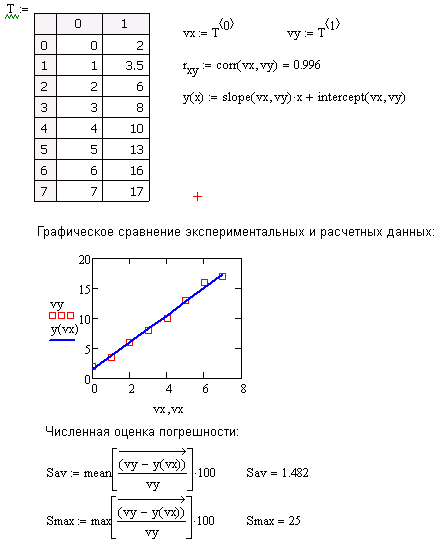
\includegraphics{old-regress-1-1.png}
\end{center}


Одной из  наиболее часто применяемых при обработке экспериментальных данных функций, является полиномиальная:
\begin{equation}
	y(x)= \sum_{i=0}^{n} a_i x^i
\end{equation}
где $a$ --- параметры. Для определения параметров полиномов используется функция \mc{regress}, которая допускает использование полинома любого порядка. Однако на практике не следует использовать степень полинома выше $n = 4$. Так как функция \mc{regress} пытается приблизить все точки данных. При недостаточном количестве экспериментальных данных высокая степень полинома может дать физически неадекватные значения.

\mc{regress(vx, vy, n)} --- возвращает вектор, требуемый \mc{interp}, чтобы найти полином порядка \mc{n}, который наилучшим образом приближает данные \mc{vx} и \mc{vy}. \mc{x} и \mc{vy} --- m-мерные векторы, содержащие значения $x$ и $y$.

\mc{interp (vs, vx, vy, x)} --- возвращает интерполируемое значение $y$, соответствующее $x$. Вектор \mc{vs} вычисляется \mc{regress} на основе данных из \mc{vx} и \mc{vy}.

\primer{Задайте экспериментальные данные в виде таблицы. Определите коэффициент корреляции. На основе этих данных двумя, вышеописанными, способами получите функцию полиномиальной регрессии, описывающую экспериментальные данные. Графически и численно определите точность полученной функции регрессии.}



Нелинейная регрессия --- эти функции используются, когда зависимость между данными близка к виду наиболее распространенных нелинейных функций: синуса, экспоненты или др. Для этих наиболее распространенных на практике нелинейных зависимостей в Mathcad встроены функции: 
\begin{itemize}
	\item \mc{expfit(x, y, g)} --- регрессия  экспоненциальной функцией $y(x)=a e^b x+c$;
	\item \mc{lgsfit(x, y, g)} --- регрессия логистической функцией $y(x)=a/(1+b e^{-c x})$;
	\item \mc{sinfit(x, y, g)} --- синусоидальная регрессия $y(x)=a sin(x+b)+c$;
	\item \mc{pwrfit(x, y, g)} --- регрессия степенной функцией $y(x)=a x^b+c$;
	\item \mc{logfit(x, y, g)} --- регрессия логарифмической функцией $f(x)=a\ ln(x+b)+c$;
\end{itemize}

Параметры \mc{x} и \mc{y} приведенных функций соответствуют векторам координат эмпирических данных. В параметре \mc{g} содержится вектор начальных приближений \mc{(a, b, c)}. Для нахождения корней Mathcad использует алгоритмы численной оптимизации, основанные на численных методах решения систем нелинейных уравнений. Численные же методы решения систем нелинейных уравнений, как вы помните, требуют задания начальных приближений к корням. В случае функций регрессии эти приближения вы передаете в векторе \mc{g}.

Обобщенная регрессия --- эти функции используются когда необходима зависимость в виде линейных комбинаций произвольных функций, ни одна из которых не является полиномом.
Задача обобщенной линейной регрессии --- ответить на следующий вопрос: какие значения должны принимать коэффициенты $a_0, a_1, ..., a_N$, чтобы функция $F(x)$, являющаяся линейным сочетанием $N+1$ произвольной функции $f_0(x), f_1(x),\\ ..., f_N(x)$ (то есть  $F(x)=a_0 f_0(x)+a_1 f_1(x)+ ... + a_N f_N(x)$), проходила между экспериментальными точками так, чтобы сумма квадратов расстояний от точек до кривой $F(x)$ была минимальной?

В Mathcad для вычисления обобщенной линейной регрессии служит встроенная функция \mc{linfit(x, y, F)}, где \mc{x} и \mc{y} --- векторы экспериментальных данных, \mc{F} --- векторная функция, содержащая в качестве элементов функции, входящие в линейное сочетание.

\primer{Задайте произвольный набор данных $y$ и $x$. Определите коэффициент корреляции данного набора данных. С помощью функции \mc{linfit} определите вид линейной зависимости между $y$ и $x$. В качестве функции используйте выражение
	$F(x)=a_0 \sin(x) + a_1 \cos(2x)+a_2 \sqrt[3]{x} + a_3 x$
	Графически и численно определите точность полученной функции регрессии.}
%пример решения

В случае, если необходимо найти коэффициенты $a_0, a_1, ..., a_N$ для следующей функции $F(x)= f_0(a_0, x) + f_1(a_1,x) +... + f_N(a_N,x)$, зависимость будет уже нелинейной по параметрам, соответственно функция \mc{linfit} уже не подойдет. Для этих целей в Mathcad есть встроенная функция \mc{genfit(x, y, g, F)}. В качестве аргументов данная функция принимает следующие параметры: \mc{x}, \mc{y} --- вектор экспериментальных данных; \mc{g} --- вектор начальных приближений для неизвестных параметров;
\mc{F(x, A)} --- описывающая экспериментальную зависимость функция, параметры которой должны быть рассчитаны.
 
\primer{}
%пример решения
Из всех встроенных функций регрессии \mc{genfit} является наиболее универсальной и может быть использована для любых функций. Однако для нелинейных по параметрам функций огромное влияние на точность расчета оказывает начальное приближение  \mc{g} для искомых параметров. Поэтому при возможности лучше привести функцию к линейному виду.

\begin{wrapfigure}{r}{0.6\textwidth} 
	\begin{tikzpicture}
	\tikzset{
		show curve controls/.style={
			decoration={
				show path construction,
				curveto code={
					\draw [blue, dashed]
					(\tikzinputsegmentfirst) -- (\tikzinputsegmentsupporta)
					node [at end, cross out, draw, solid, red, inner sep=2pt]{};
					\draw [blue, dashed]
					(\tikzinputsegmentsupportb) -- (\tikzinputsegmentlast)
					node [at start, cross out, draw, solid, red, inner sep=2pt]{};
				}
			}, decorate
		}
	}
	
	%\draw [gray!50]  (0,0) -- (1,1) -- (3,1) -- (1,0)  -- (2,-1) -- cycle;
	%\draw [show curve controls] plot [smooth cycle] coordinates {(0,0) (1,1) (3,1) (1,0) (2,-1)};
	%\draw [red] plot [smooth cycle] coordinates {(0,0) (1,1) (3,1) (1,0) (2,-1)};
	
	\draw [gray!50, xshift=4cm]  (0,0) -- (1,1) -- (3,1.3) -- (5,2) -- (7,1.5);
	\draw [cyan, xshift=4cm] plot [smooth, tension=1] coordinates { (0,0) (1,1) (3,1.3) (5,2) (7,1.5)};
	\draw [show curve controls,cyan, xshift=4cm] plot [smooth, tension=1] coordinates { (0,0) (1,1) (3,1.3) (5,2) (7,1.5)};
	\end{tikzpicture}
	\caption{Схематическое изображение аппроксимацией сплайном}\label{fig:old.regress.spline}
\end{wrapfigure}

В случае обработки точных данных, представленных в дискретном виде (например в случае численного решения дифференциальных уравнений) удобнее использовать сплайны. Сплайн представляет из себя кусочную функцию, составленную из полиномов какой-либо степени (\ref{fig:old.regress.spline}). Результирующая функция будет строго проходить через экспериментальные точки. Сплайны неприемлемо применять для аппроксимации экспериментальных данных в связи с тем, что погрешности эксперимента будут вносить существенное влияние на результирующую функцию.



Вопросы для самоконтроля:
\begin{enumerate}
\item Что такое регрессионный анализ?
\item Что такое коэффициент корреляции?
\item Какие виды функций регрессии существуют, в чем их различие?
\item Какие функции решения уравнения с одним неизвестным и системы уравнений используются в MathCad?
\item Что является результатом решения системы нелинейных уравнений?
\item Какие символы должны использоваться в качестве знаков равенства или неравенства при записи уравнений в вычислительном блоке \mc{Given-Find}?
\end{enumerate}